\documentclass[12pt,a4paper,openright,twoside]{book}
\usepackage[utf8]{inputenc}
\usepackage{disi-thesis}
\usepackage{code-lstlistings}
\usepackage{notes}
\usepackage{shortcuts}
\usepackage{acronym}
\usepackage{svg}

\school{\unibo}
\programme{Corso di Laurea in Ingegneria e Scienze Informatiche}
\title{Sviluppo di un'Interfaccia Grafica per Software Simulativi Complessi mediante GraphQL e KotlinJS}
\author{Tiziano Vuksan}
\date{\today}
\subject{Programmazione ad Oggetti}
\supervisor{Dott. Danilo Pianini}
\cosupervisor{Dott. Angelo Filaseta}
\session{IV}
\academicyear{2023-2024}

% Definition of acronyms
%\acrodef{IoT}{Internet of Thing}
\acrodef{API}{Application Program Interface}
\acrodef{DOM}{Document Object Model}
\acrodef{REST}{Representational State Transfer}
\acrodef{URL}{Uniform Resource Identifier}
\acrodef{UI}{User Interface}
\acrodef{JVM}{Java Virtual Machine}


\mainlinespacing{1.241} % line spacing in mainmatter, comment to default (1)

\begin{document}

\frontmatter\frontispiece

\begin{abstract}	
Max 2000 characters, strict.
\end{abstract}

%\begin{dedication} % this is optional
%Optional. Max a few lines.
%\end{dedication}

%\begin{acknowledgements} % this is optional
%Optional. Max 1 page.
%\end{acknowledgements}

%----------------------------------------------------------------------------------------
\tableofcontents   
\listoffigures     % (optional) comment if empty
\lstlistoflistings % (optional) comment if empty
%----------------------------------------------------------------------------------------

\mainmatter

%----------------------------------------------------------------------------------------
%----------------------------------------------------------------------------------------
\chapter{Introduzione}
\label{chap:introduction}
%----------------------------------------------------------------------------------------

\section{Contesto}
\subsection{Simulazione}
\subsection{Alchemist}
\section{Motivazione}
\section{Obiettivi}
%----------------------------------------------------------------------------------------

%----------------------------------------------------------------------------------------
\chapter{Analisi}
%I suggest referencing stuff as follows: \cref{fig:random-image} or \Cref{fig:random-image}
%\begin{figure}
%	\centering
%	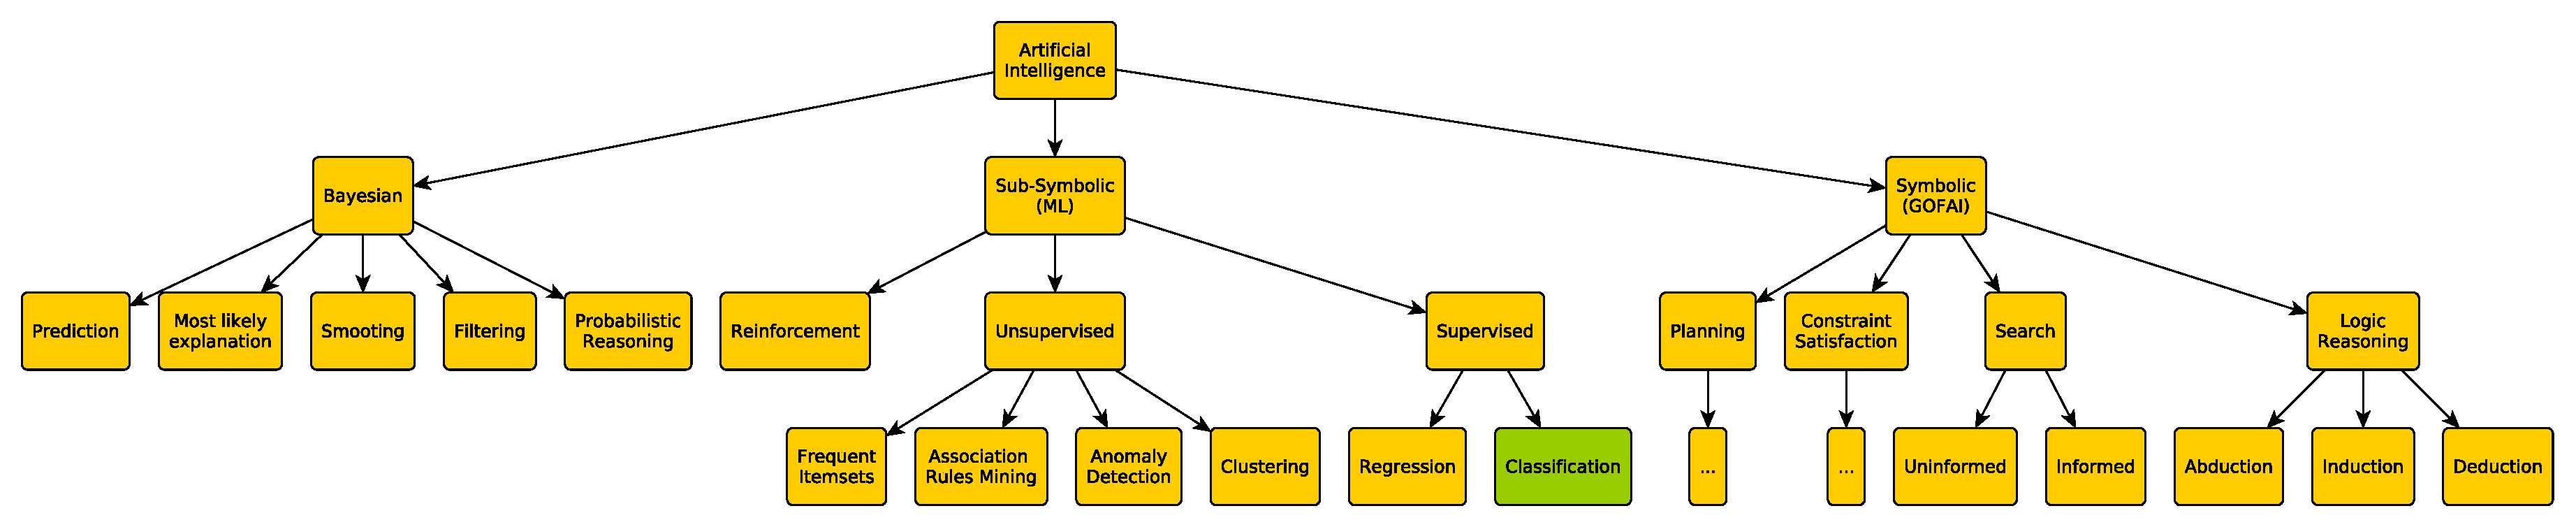
\includegraphics[width=.8\linewidth]{figures/random-image.pdf}
	%\caption{Some random image}
	%\label{fig:random-image}
%\end{figure}

\section{Analisi dei requisiti}

Lo scopo principale del progetto è la realizzazione di una interfaccia web (quindi interpretabile da un qualsiasi browser moderno) che permetta l'interazione con il sistema software di simulazione
\textit{Alchemist} in modo intuitivo e \textit{user-friendly}. Il compito dell'applicativo sarà quindi quello di comunicare, attraverso apposite \ac{API}, con l'infrastruttura server preesistente e presentare in seguito a cambiamenti della simulazione in corso o a richieste da parte dell'utente, un'interfaccia grafica che ne rappresenti i risultati.
\subsection{Requisiti funzionali}
\begin{itemize}
	\item L'applicativo dovrà presentare un interfaccia grafica all'interno di un web browser.
	\item L'applicativo dovrà interfacciarsi con l'infrastruttura GraphQL già presente all'interno del progetto.
	\item In una tipica simulazione di \textit{Alchemist} (come discusso nel paragrafo) sono presenti dei nodi. L'applicativo quindi dovrà essere in grado di rappresentare in un piano bidimensionale la posizione di tali nodi all'interno di un contesto grafico. Ciò implica ovviamente che con l'evolversi della simulazione il contesto grafico debba essere aggiornato. \footnote{Date le diverse \textit{incarnation} e i diversi possibili scenari che \textit{Alchemist} può modellare non è detto che i nodi cambino di posizione.}
	\item Ogni nodo contiene diverse proprietà, reazioni, concentrazioni etc. L'interfaccia dovrà permettere di ispezionare il contenuto di ciascun nodo. 
	\item L'interfaccia dovrà controllare lo stato attuale della simulazione. Ciò vuol dire poterla eseguire o mettere in pausa.
\end{itemize}

\subsection{Requisiti non funzionali}
\begin{itemize}
	\item Interagendo con l'interfaccia, non si devono verificare tempi di risposta eccessivi. Per esempio se l'utente decide di ispezionare un nodo, il recupero di tali informazioni deve essere presentato in tempi ragionevoli.
	\item L'applicativo deve essere compatibile con un ambiente multipiattaforma.
	\item L'architettura delle componenti grafiche deve essere estendibile e facilmente modificabile.
\end{itemize}

\subsection{Architettura API GraphQL}
Prima di analizzare il funzionamento principale dell'architettura server esistente è utile capire brevemente le motivazioni dietro l'utilizzo di GraphQL e il contesto per il quale nasce. GraphQL\footnote{\url{https://graphql.org/foundation/}} è un linguaggio di interrogazione per le \ac{API} che offre una sintassi flessibile e potente per recuperare dati da un server, creato da Facebook nel 2012 come alternativa all'esistente architettura \ac{REST}. Evidenziamo quindi i punti di forza più pertinenti:
\begin{itemize}
	\item \textbf{Flessibilità nelle query}: i client possono richiedere esattamente i dati di cui hanno bisogno, evitando di occupare, nelle richieste di dati, più banda di rete del necessario. Con questo linguaggio vengono risolti quindi i problemi di \textit{over-fetching} e \textit{under-fetching}.
	\item \textbf{Unica endpoint}:  mentre nelle architetture di tipo \ac{REST} i dati sono esposti tramite endpoint dedicati che corrispondono ciascuno a una risorsa specifica (identificati tramite un \ac{URL} univoco), in GraphQL l'interrogazione dei dati avviene tramite un unico \textit{endpoint}.
	\item \textbf{Tipizzazione forte}: GraphQL offre una tipizzazione forte dei dati, consentendo ai client di conoscere in anticipo i tipi di dati che riceveranno in risposta alle loro query. Questo porta a un maggiore controllo e previsione durante lo sviluppo delle applicazioni.
\end{itemize}
È facile quindi notare come questo linguaggio semplifichi lo sviluppo di applicazioni frontend.

L'interazione con i dati avviene attraverso tre operazioni: 
\begin{itemize}
	\item \textbf{Query}: operazione di lettura per ottenere un tipo determinato di dato dal server.
	\item \textbf{Mutation}:  operazione di scrittura per modificare uno o più dati sul server.
	\item \textbf{Subscription}: operazione per ricevere i cambiamenti di uno o più tipi di dati in tempo reale.
\end{itemize}

\subsection{Web Server GraphQL}

Al centro delle operazioni GraphQL c'è uno schema che definisce tutti i tipi di dati disponibili e le relazioni che ci sono tra di essi, oltre che alle operazioni che possono essere eseguite. La natura intrinseca dello schema garantisce che fra client e server ci sia un meccanismo di \textit{type safety} che previene errori legati a richieste che non sono compatibili. Per questo, uno strumento molto utile messo a disposizione dal web server, accessibile tramite l'\textit{endpoint} \texttt{/graphiql}, è il \textit{playground} GraphiQL. Qui è possibile effettuare e verificare \textit{ex-ante} il risultato delle operazioni che si intendono fare prima che queste vengano usate per generare le classi associate durante la fase di compilazione del progetto. Questo processo, per lo sviluppo di un qualsiasi applicativo client che si appoggia su queste \ac{API}, permette allo sviluppatore di validare ogni singola operazione che verrà utilizzata all'interno dell'applicativo che si intende sviluppare.

\subsection{Rendering del contesto grafico}
È importante sottolineare come le prestazioni siano un fattore decisivo nella scelta delle tecniche per rappresentare l'ambiente della simulazione.
In questo contesto, prestazioni ottimali assicurano un'esperienza utente fluida e soddisfacente. È per questo motivo che la scelta di disegnare i nodi della simulazione di \textit{Alchemist} direttamente all'interno di un elemento di tipo \textit{canvas } HTML prevale rispetto alla rappresentazione tramite elementi \ac{DOM}. Nell'ipotesi in cui si decidesse di rappresentare ciascun nodo con un elemento del DOM (e.g. \texttt{div}), il \textit{rendering} risulterebbe oneroso, perché ogni elemento \ac{DOM} aggiunto alla pagina web richiederebbe risorse di sistema per essere gestito e disegnato dal browser. Con un considerevole numero di nodi, oltretutto aggiornati frequentemente, questo metodo causerebbe solo un deterioramento delle prestazioni. Inoltre, utilizzando un \textit{canvas}, si ha maggiore flessibilità nel disegno dei nodi e nel loro comportamento. Si può disegnare senza nessun vincolo una qualsiasi forma o figura, applicare trasformazioni ed effetti visivi senza doversi occupare delle restrizioni del \ac{DOM}. D'altro canto, agli elementi del \ac{DOM} possono essere collegati dei \textit{listener}, funzioni associate a un determinato tipo di evento, come un click o il movimento del mouse. Sebbene questo vantaggio, il \textit{canvas} torna più utile in questa situazione perché offre la possibilità di implementare interazioni più complesse, come per esempio lo zoom del contesto (modifica della scala) o la traslazione dell'intera area di disegno.
Il processo di rendering dei nodi sul \textit{canvas} è illustrato in figura \cref{fig:rendering-graphics}. Inizialmente, il sistema apre una connessione con il Client GraphQL e si iscrive alla richiesta di invio dei nodi. Il server accetta la richiesta d'iscrizione e invia dati fino a quando la \textit{subscription} non viene cancellata o completamente consumata. A ogni iterazione il Web Client ridisegna i nodi nel \textit{canvas}.
A ogni fase della simulazione i nodi possono cambiare di posizione o meno, in base al tipo di simulazione che è in esecuzione. 
\begin{figure}
	\centering
	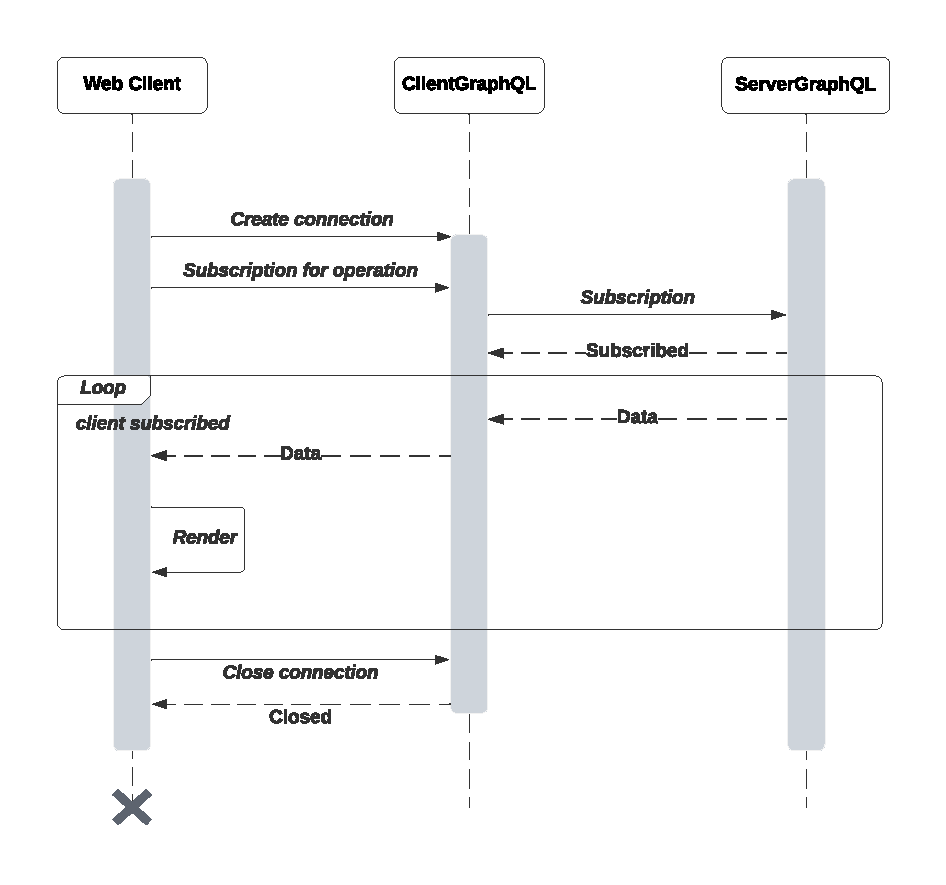
\includegraphics[width=.65\linewidth]{imgs/Rendering_Diagramma_Sequenza.pdf}
	\caption{Diagramma di sequenza del rendering dei nodi a seguito di una \textit{subscription}}
	\label{fig:rendering-graphics}
\end{figure}

\subsection{Progetto multiplatform}
Kotlin Multiplatform è una tecnologia che permette lo sviluppo di codice Kotlin condivisibile tra diverse piattaforme, come per esempio Android, iOS, web e desktop. Questo significa che è possibile utilizzare lo stesso codice Kotlin per creare applicazioni native per diverse piattaforme, riducendo la necessità di scrivere e mantenere codice separato per ciascuna piattaforma. 
Caratteristica dei progetti multipiattaforma è che sono composti dai cosiddetti \textit{source sets}: insiemi di codice sorgente specifico della piattaforma a cui si riferiscono. Generalmente è sempre presente il modulo comune, detto ``common code''. Questo modulo contiene il codice condiviso che può essere utilizzato su tutte le piattaforme. Ad accompagnarlo quindi sono altri \textit{source sets} aggiuntivi, compilati per target diversi come \ac{JVM}, JavaScript o nativo. Nel caso dello sviluppo di una applicazione in-browser il progetto potrebbe includere i seguenti \textit{source set}:
\begin{itemize}
	\item \textbf{Common Source Set}: Codice condiviso che può essere utilizzato su tutte le piattaforme target.
	\item \textbf{JVM Source Set}: Codice destinato al target \ac{JVM}. Da qui può essere gestita una componente server dal quale sarà accessibile l'interfaccia grafica.
	\item \textbf{JavaScript Source Set}: Codice destinato al target JavaScript. Qui viene definita la struttura e il comportamento dell'interfaccia grafica vera e propria.
\end{itemize}

\section{Analisi e Modello del Dominio}
Uno dei requisti di questo applicativo verte sul bisogno di creare una piattaforma web tale da impiegare le \ac{API} esposte dall'infrastruttura GraphQL fornita. Pertanto non esiste una comunicazione diretta tra il web client e la simulazione di \textit{Alchemist}. La gestione dell'accesso e del recupero dei dati dal modello della simulazione è affidata alla componente server, che, al contempo, fornisce anche un punto di accesso ai client che richiedono tali dati.
Il client-web quindi comprende un modulo (nell'immagine ClientGraphQL) che si pone da interfaccia tra l'applicazione web vera e propria e l'\textit{endpoint } sulla quale la componente server utilizzerà per ricevere richieste e mandare risposte (\textit{endpoint} \texttt{/graphql}). 
Il compito del client-web quindi sarà quello di utilizzare le operazioni possibili (\textit{query}, \textit{mutation} e \textit{subscription}) e utilizzare i risultati per rappresentarli graficamente.

\textit{Alchemist} presenta già altri moduli che rappresentano l'ambiente di simulazione, implementati con tecnologie differenti a quelle che verranno proposte successivamente in questo elaborato. Il modulo specifico che viene avviato per rappresentare la simulazione dipende dalla configurazione con cui viene avviato l'intero software. Di conseguenza, è opportuno che l'interfaccia web e la componente server vengano avviate esclusivamente attraverso una specifica configurazione della simulazione.



%----------------------------------------------------------------------------------------

%----------------------------------------------------------------------------------------
\chapter{Design}

%You may also put some code snippet (which is NOT float by default), eg: \cref{lst:random-code}.

%\lstinputlisting[float,language=Java,label={lst:random-code}]{listings/HelloWorld.java}

\section{Layout dell'interfaccia}
\subsection{I componenti}
\section{Architettura client}
%----------------------------------------------------------------------------------------

%----------------------------------------------------------------------------------------
\chapter{Implementazione e Verifica}

\section{Componenti grafici}

\section{Uso di Redux}

\section{Binding dei dati}

\section{Esecuzione di operazioni GraphQL}

\section{Verifica}
%----------------------------------------------------------------------------------------

%----------------------------------------------------------------------------------------
\chapter{Conclusione}

\section{Lavori futuri}
%----------------------------------------------------------------------------------------

%----------------------------------------------------------------------------------------
% BIBLIOGRAPHY
%----------------------------------------------------------------------------------------

\backmatter

\nocite{*} % comment this to only show the referenced entries from the .bib file
\bibliographystyle{alpha}
\bibliography{bibliography}

\end{document}